\documentclass{article}
\usepackage{hyperref}
\usepackage {graphicx, amsmath}
\usepackage[margin=1.0in]{geometry}
\title{F24 CSE220 Lab2}
\author{
  Andrew Bruce \\ \href{mailto:acbruce@ucsc.edu}{acbruce@ucsc.edu} \and
  Mohit Agrawal \\ \href{mailto:mmagrawa@ucsc.edu}{mmagrawa@ucsc.edu}
}

\begin{document}
\maketitle

\section*{Part1}
\subsection*{IPC}
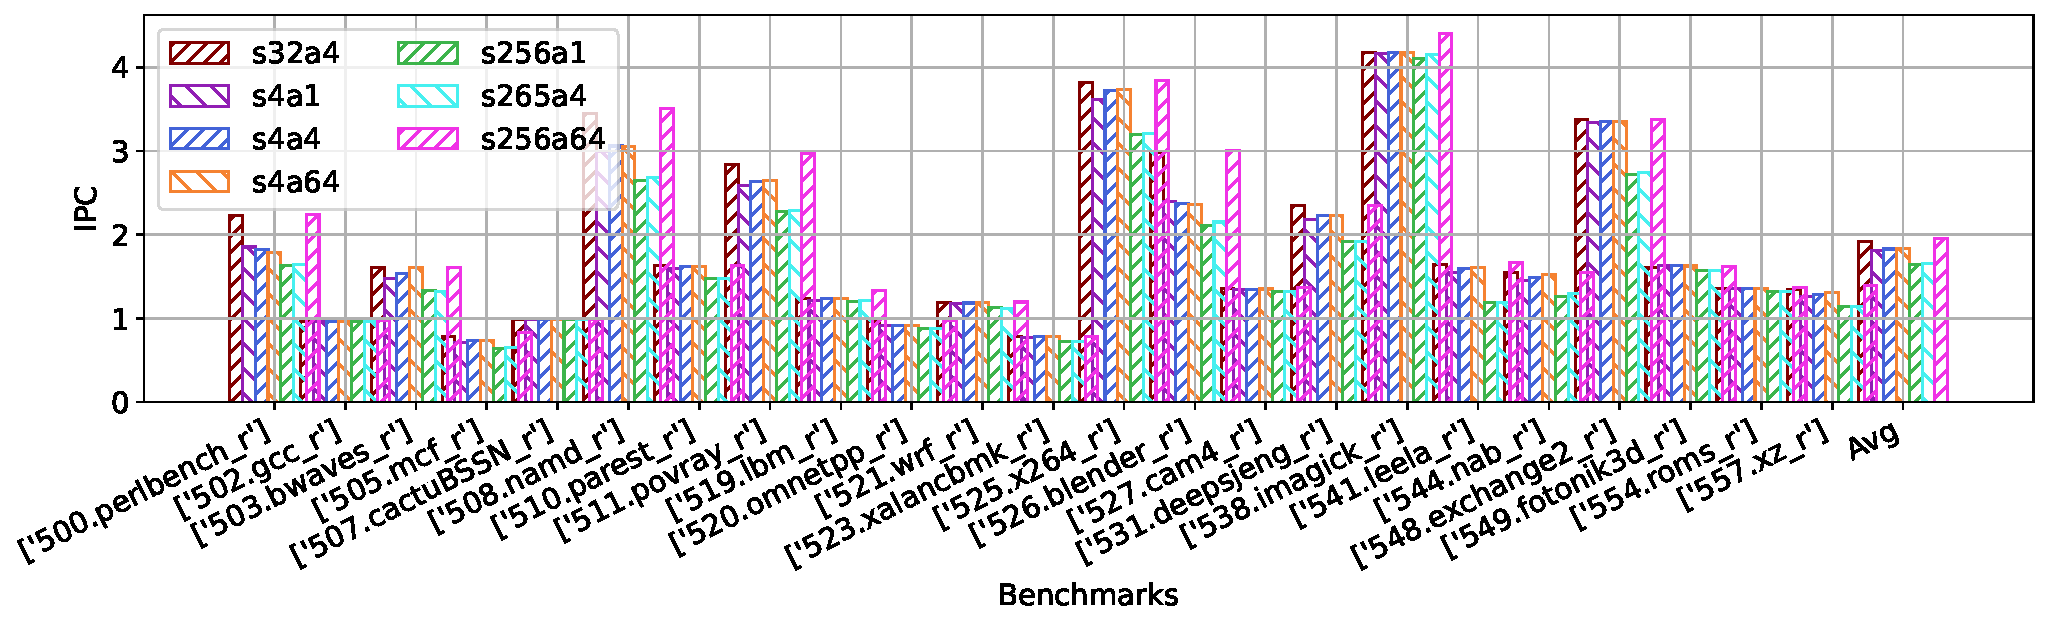
\includegraphics[width=\textwidth]{Part1/IPC.pdf}.
In this plot increasing both the size and assosiativity of the cache increases the IPC for almost every single test. Increasing the associativity from 1 to 4 was not as effective as increasing the size from 4kb to 256kb at increasing IPC.
\subsection*{DCache miss rate}
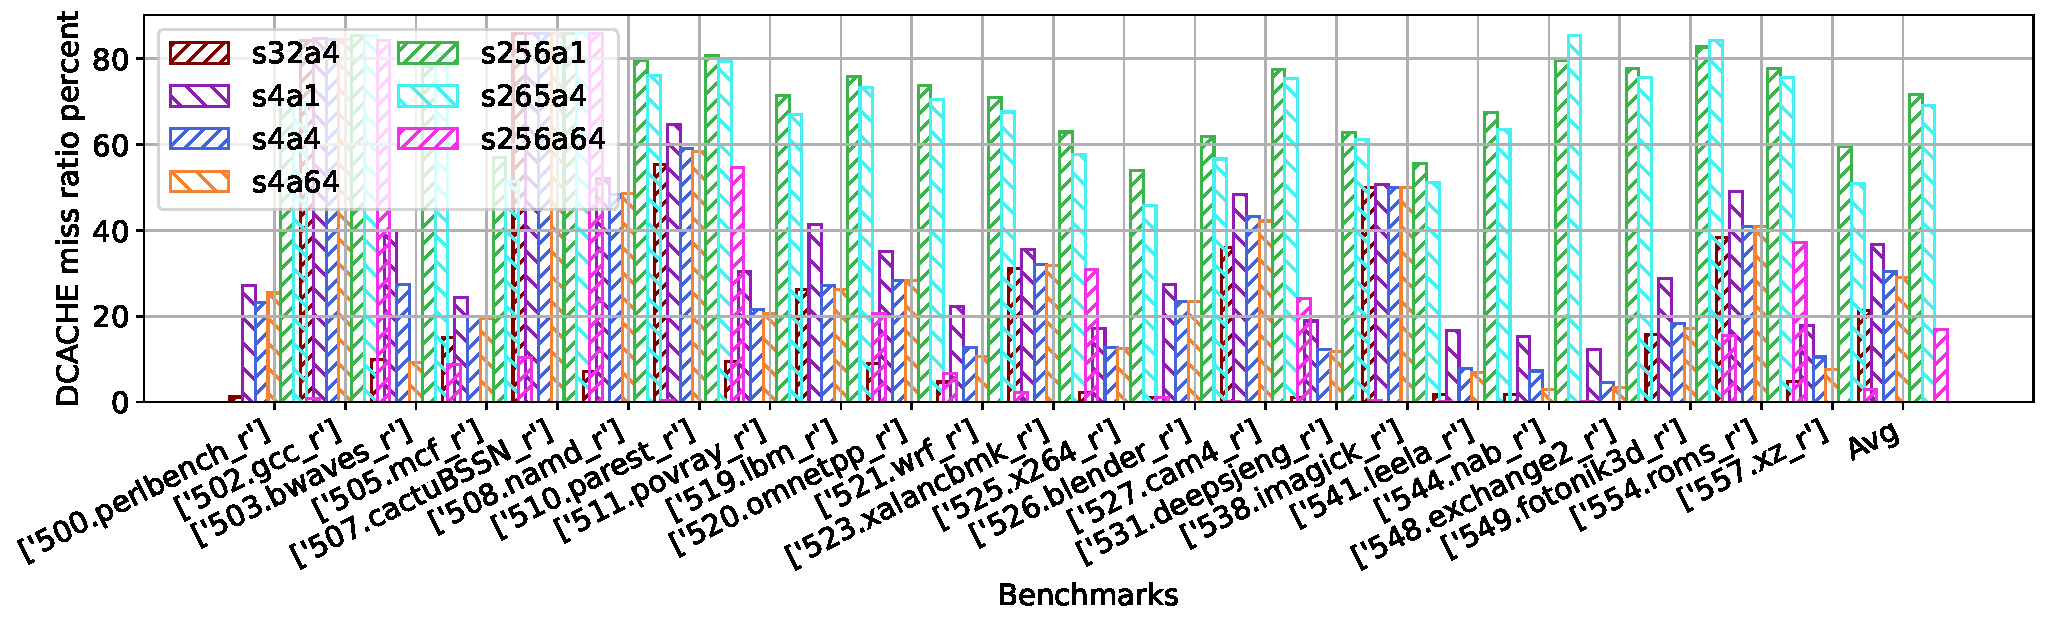
\includegraphics[width=\textwidth]{Part1/DCACHE.pdf}.
Outside of GCC and cactuBSSN, increasing the cache size to 256 kb universally decreased the miss ratio of the dcache. Increasing assosiativity also lowered the miss ratio.
\section*{Part3}
\subsection*{DCache miss types}
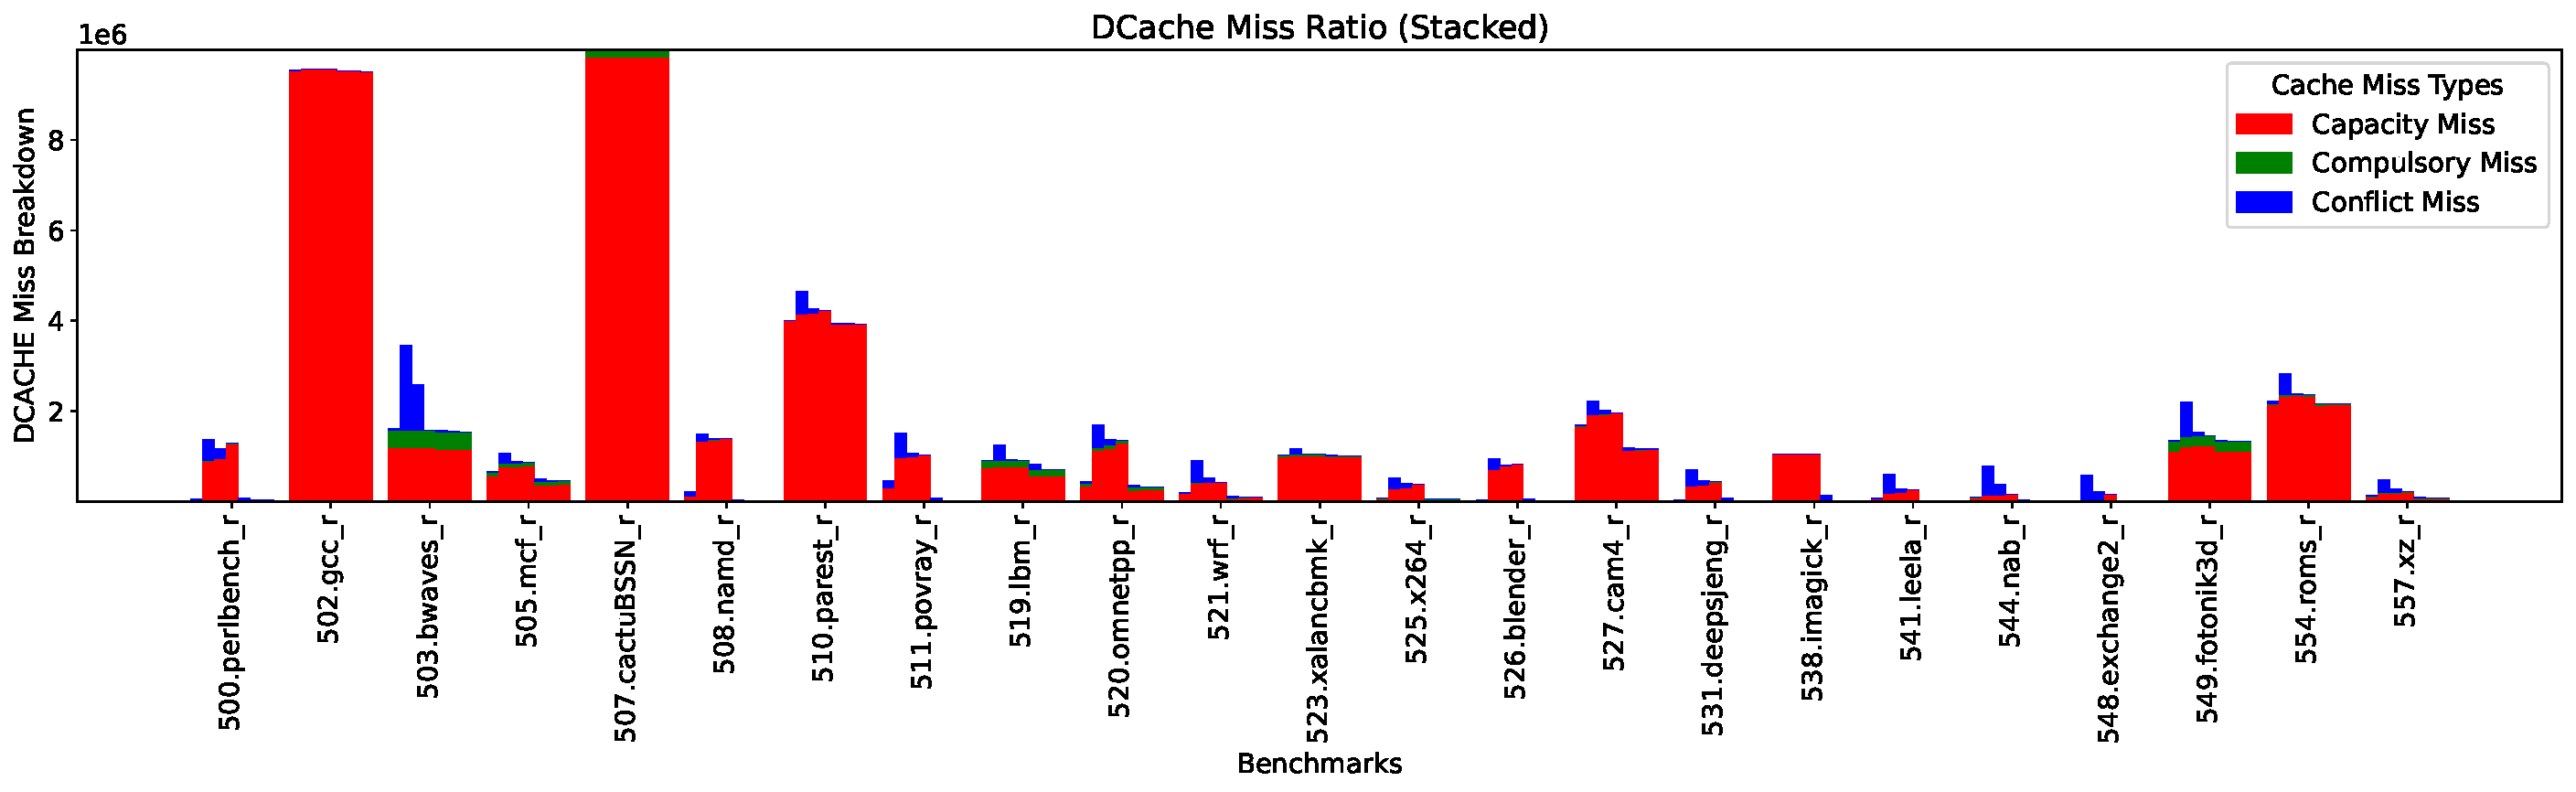
\includegraphics[width=\textwidth]{Part3_4/DCACHE_MISS_STACKED.pdf}.
This graph is the same as the dcahce miss rate but colored based on their type. The vast majority of misses are conflict misses. Compulsary misses are usually the least common, possibly because they only happen once per block.\\
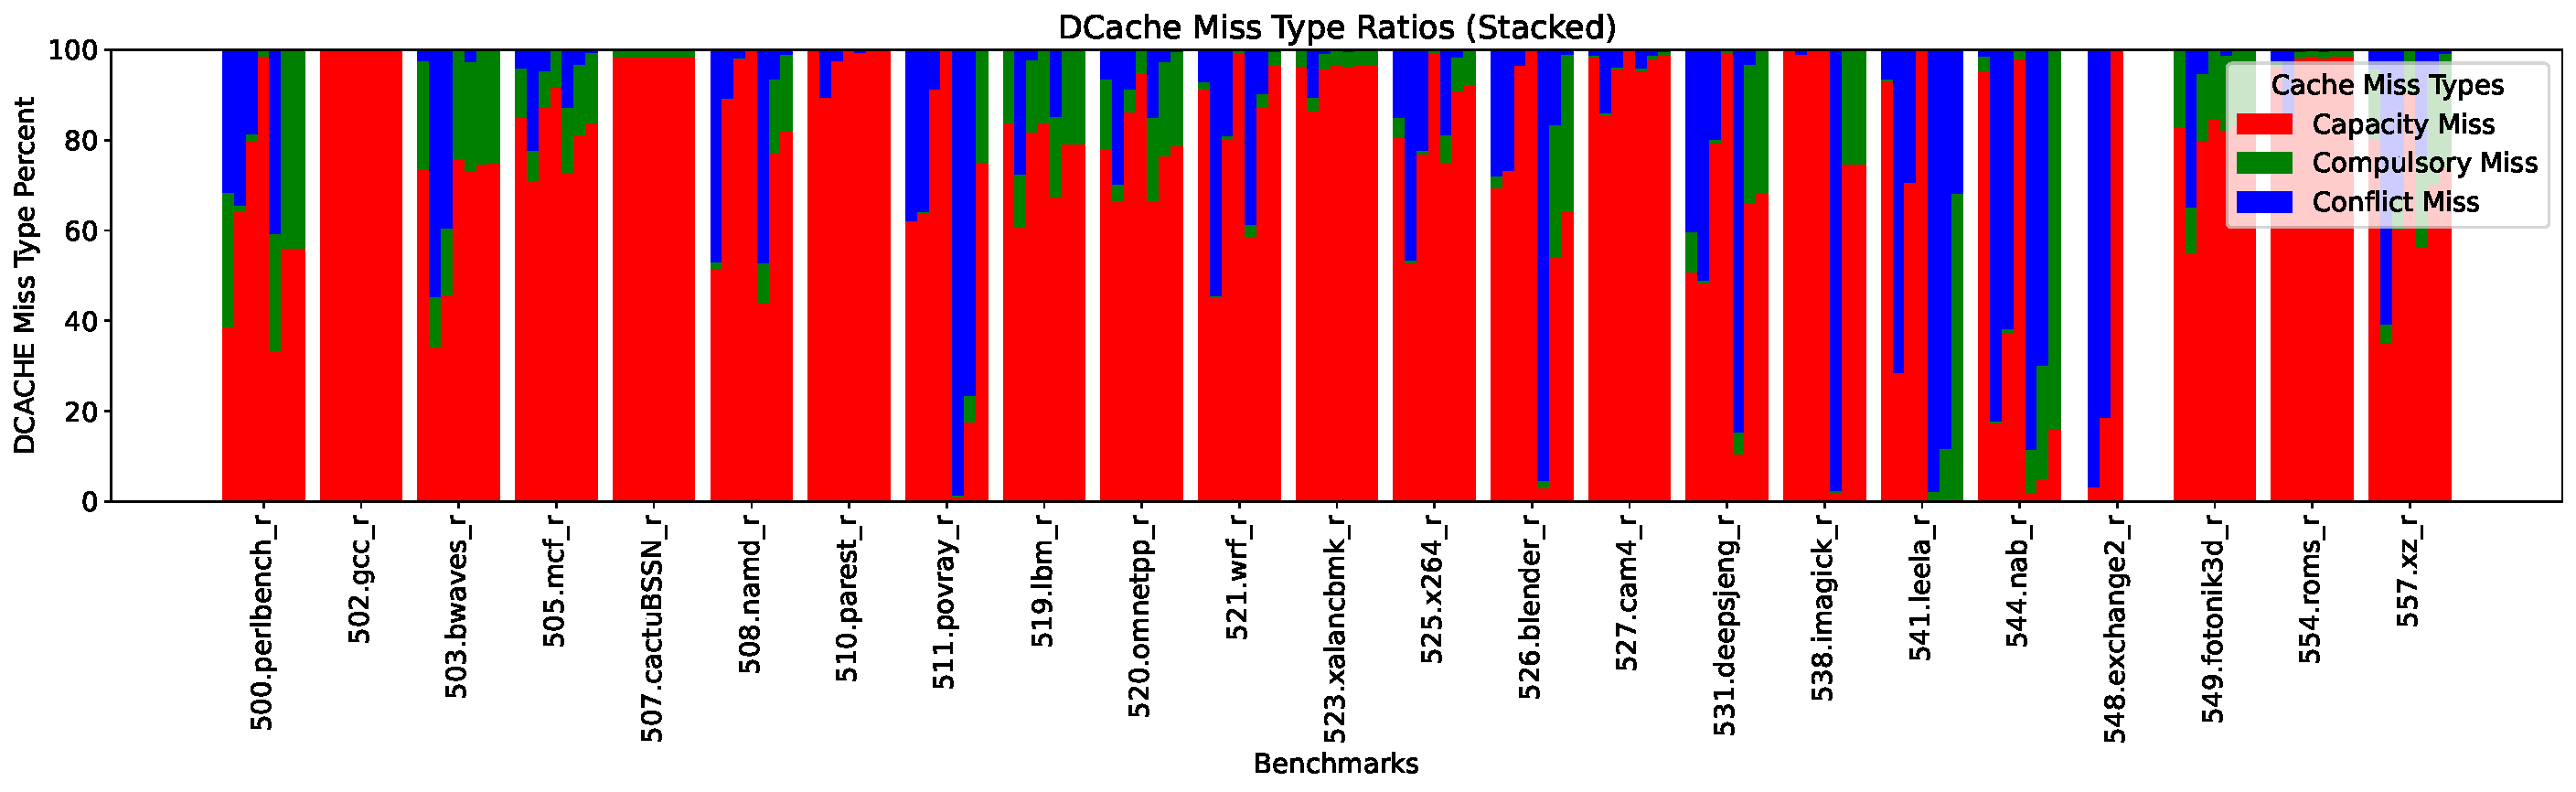
\includegraphics[width=\textwidth]{Part3_4/DCACHE_MISS_STACKED_RATIO.pdf}.
This graph shows the ratio of the types for each type.
\end{document}

